Here we present \textit{easyReporting}, an \textit{R6} \footnote{\url{https://adv-r.hadley.nz/r6.html}}\footnote{\url{https://cran.r-project.org/web/packages/R6/index.html}} class\footnote{\url{https://en.wikipedia.org/wiki/Class_(computer_programming)}} developers to integrate a reproducible research layer inside their software products, as well as lazy analysts to speed up their report production without learning the \textit{rmarkdown} language.

In such a way, thanks to minimal additional efforts of developers, the end user has available an \textit{rmarkdown} file within all the source code generated during the analysis, divided into \glspl{cc} ready for the compilation.

\begin{figure}[H]
\centering
\includegraphics[width=\textwidth, keepaspectratio]{img/rr/scheme.pdf}
\caption[Reproducible Computational Research illustration]{A general illustration of Reproducible Computational Research concept. Raw data can be analysed with R code, producing plots, tables and additional caching database files. All together, R code, data and results can be inserted in an enriched document, which can be added as supplementary material to a valuable published article.}
\label{fig:rrscheme}
\end{figure}

Once manually edited with comments and descriptions the file can be compiled to produce an enriched document within input data, source code and output results.

A so final document can be attached to the publication of the analysis as supplementary material, helping the interested community to entirely reproduce the computational part of work (figure \ref{fig:rrscheme}). 

The package is accessible at the following link:\\ \href{https://github.com/drighelli/easyreporting}{https://github.com/drighelli/easyreporting} 

\subsubsection{General Description and Initialization}

The class can to be imagined as a schematic representation of the \textit{rmarkdown} file (\textit{report}), indeed 
its attributes represent the \textit{report} characteristics, which are typically inserted in the header of the file.
But our class methods are not only for the attributes manipulations, but also for insertion of \glspl{cc}, comments and section titles inside the \textit{report}.

As any typical class, before of using it, \textit{easyReporting} requires to be initializated with the \lstinline!new! command, passing as mandatory arguments the \textit{path} and the name of the file as \lstinline!filenamepath! and a title as \lstinline!mainTitle!.
Additionally, an \lstinline!author! and the \lstinline!documentType! can be specified.

When initializing, the class automatically creates the \textit{report} with the entire specified folder tree, setting up the header of it and declaring the general options for the \textit{rmarkdown} file.
If \textit{rmarkdown} personal options (see figure \ref{fig:knitropts} for a list of available options) are required, before creating an instance of the class, it is possible to use the \lstinline!makeOptionsList! function, and then assigning the output to the \lstinline!optionsList! argument of the class \lstinline!constructor!.

\begin{figure}[H]
\centering
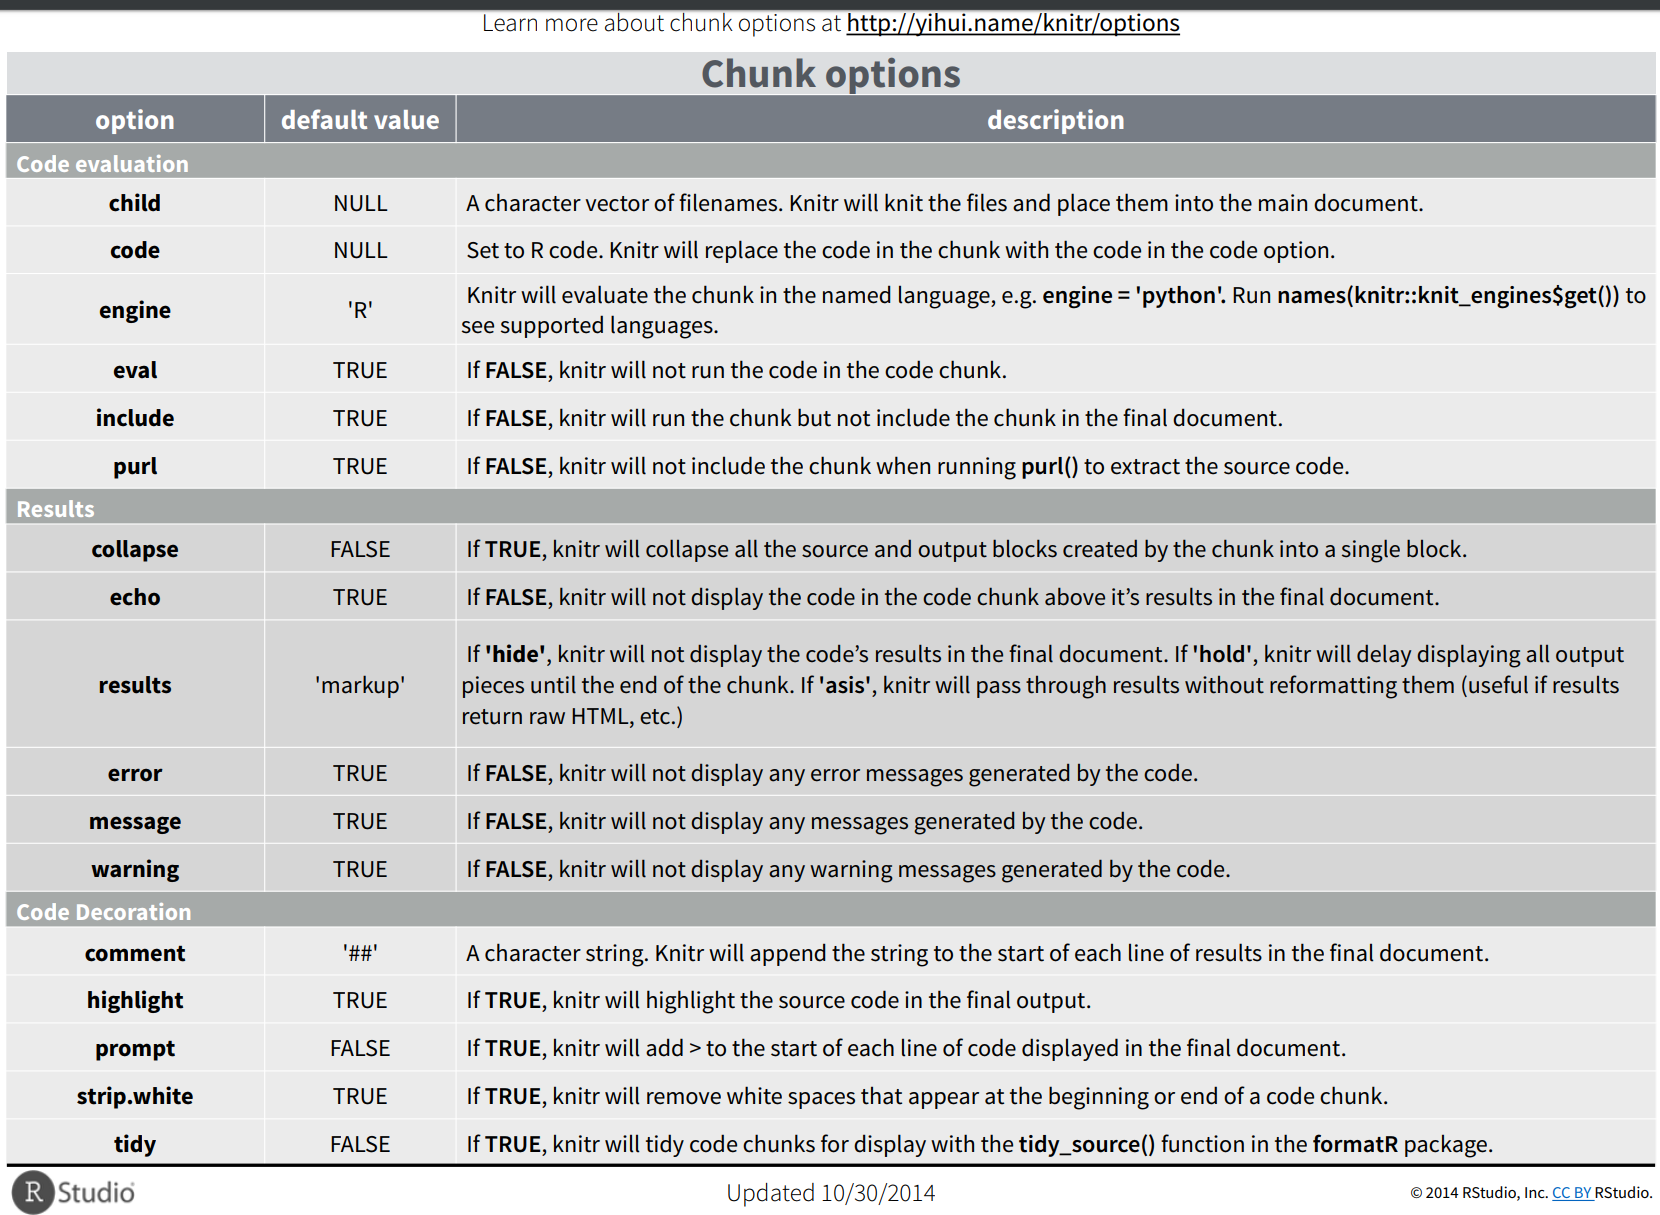
\includegraphics[width=\textwidth, keepaspectratio]{img/rr/knitropts.png}
\caption[knitr options]{A schematic table of options available using knitr and rmarkdown packages.}
\label{fig:knitropts}
\end{figure}



\subsubsection{Class Methods}

The class is provided of several methods for \textit{rmarkdown} \gls{cc} construction.

Once an \textit{easyReporting} instance is available, with \lstinline!mkdTitle! it is possible to insert six levels of titles, by setting the parameters \lstinline!title! and \lstinline!level!.
It is also possible to add natural language comments with \lstinline!mkdGeneralMsg!.

When working with \glspl{cc}, two main choice are available.
The first one gives the possibility to construct a \gls{cc} as additional steps, by using first the \lstinline!mkdCodeChunkSt!, then adding variable assignment and/or function calling with \lstinline!mkdVariableAssignment! or \lstinline!mkdGeneralMsg!, and finally closing the \gls{cc} with \lstinline!mkdCodeChunkEnd!.

In particular, when starting a \gls{cc} with \lstinline!mkdCodeChunkSt!, it is possible to assign a specific \lstinline!optionList! and/or a \lstinline!source.files.list! to be added to that \gls{cc}.

Otherwise it is possible to create an entire \gls{cc} just with \lstinline!mkdCodeChunkComplete! and assigning the entire function call as a \lstinline!message!.
This way of working is really useful with \lstinline!function! creation, where inside a developed function a simple recursive call with parameters assignment can be done as a single \lstinline!message!.




